\chapter{Historical Analysis}\label{chp-his-analysis}
If you want to predict the future, go look into the past\footnote{In business schools, we usually only learn about things that have happened in the past; here we also analyse what is happening now and what will possibly happen in the near future.}. 

In this chapter, we first seek to go back in time machine to take a retrospective view of the history concerning related fields, from a combination of industrial and academic perspectives. Then, we do some analysis, analysing technologies that emerged, why they became standards and why some were unsuccessful in the end. We also state practical lessons we have learned from this history and how these have inspired our decisions, resolutions and solutions\footnote{We only talk about the technologies that are general-purpose, and have made a difference or will potentially change the world in multiple areas to a great extent. We discuss domain-specific technologies, techniques, applications and phenomena in the respective following chapters.}.
%define the core problems which inspires and unveils  
% push our thinking to get the root causes

\section{Network Protocol and Efficiency}\label{sec-his-analysis-tcp}
The ancestor of today's Internet was the ARPANET, a military project established by DARPA (the then ``ARPA'') of the US Department of Defense (DOD) in 1969. Its primary goal was to decentralise the command and control processing and switching so the communication network could survive a nuclear attack. In the beginning, ARPANET used a simplex protocol called the Network Control Program (NCP) for communication between host computers. 

In 1983, the Transmission Control Protocol / Internet Protocol (TCP/IP) suite replaced NCP as ARPANET's principal protocol, and ARPANET then became a part of the early Internet. According to statistics from different parties, TCP accounts for 60\% to 95\% of the wide-area Internet traffic. 

TCP uses a decent ``gentleman'' congestion control mechanism \cite{Chiu:1989:AIMD} that guarantees long-term fairness among competing connections. It does not rely on the routers (intermediate nodes) to give any feedback information about network conditions to the source. This end-to-end elegency\footnote{Similar scenarios also exist in Artificial Intelligence and Deep Learning: if an end-to-end solution is developed, it is more likely to be shortly accepted and widely deployed to solve general or domain-specific real-world problems.} reminds of another story. 

Ethernet/TCP/IP is adequate in many data transmission scenarios, but inadequate for Quality of Service (QoS) guaranteed telecommunication applications. Thus, intermediate network nodes were considered to be used to provide feedback regarding congestion status. In the 1990s the Asynchronous Transfer Mode (ATM) was popular as a protocol stack that worked on multiple layers that actualised such mechanism. At that time, ATM attracted much investment and research interest. However, it almost died and was replaced by Ethernet/IP in most public networks at the beginning of this millennium. Below we try to list some reasons: 
% makes us recall another story (which required every node adds feedback field to imply the end the congestion status) in the evolution of the Internet protocol stack.

\begin{description}
	\item[High Complexity and High Cost] Compared with Ethernet/IP, ATM was more expensive in terms of the required hardware and manpower for operation. It also required more time to train people to become experts. 
	\item[Weak Value Proposition] The development of statistical multiplexing technologies overshadowed the advantages of ATM. Although Ethernet/IP networks originally could not guarantee a high degree of QoS, this factor diminished over time as statistical multiplexing technologies improved.  
	\item[Weak Interoperability] Ethernet created a sustainable eco-system: it supported an open, multi-vendor and cross-platform environment; ATM did not. An existing ATM switch would probably not interoperate with one from a second vendor. This meant that after purchasing an ATM switch from one vendor, the user was locked into that supplier. 
	\item[Weak Upgradeability] It is easy to upgrade Ethernet to 100 Mbit/s, to 1Gbit/s, and even 10Gbit/s, while upgrading ATM requires all legacy software to be changed. Eventually, Ethernet won the speed race in LAN over ATM: 100BaseT Ethernet kicked out 25 Mb/s ATM in the desktop; 1Gbps/10Gbps Ethernet wiped out ATM on the campus. 
	\item[Weak Profitability to Most Parties] Only the telephone companies were active in deploying ATM networks. The reason was quite simple: to count the bits a customer generated/consumed in the established end-to-end connection conveniently and charge him accordingly.  
	\item[Slow in Touching Ground in the Market and Industrial Standardisation] Network operators would be required to change the infrastructure, since in the LAN world IP and Ethernet first took hold as the \textit{de facto} standards, and equipments based on these standards were so much simpler, easier to understand and significantly cheaper than the corresponding ATM equipments.
\end{description}

It is known to all networking professionals that Equation~\ref{throughput:formula:tcp}  below is the throughput TCP can achieve at a steady state; Equation~\ref{throughput:formula:tcp:max} is roughly the maximum throughput TCP can achieve. 
\begin{equation}\label{throughput:formula:tcp}
Throughput_{TCP} = \frac{\min\{RWND, CWND\}}{RTT}
\end{equation}
\begin{equation}\label{throughput:formula:tcp:max}
Throughput_{TCP_{max}} = \frac{RWND_{max}}{RTT}
\end{equation}
where $RWND$ is the receiver window size, $CWND$ is the congestion windows size (at the sender side), and $RTT$ is the round trip time. 

Also, theoretically we have Equation~\ref{throughput:formula:tcp2} if considering the loss rate $p$. 
\begin{equation}\label{throughput:formula:tcp2}
Throughput_{TCP} \sim \frac{1}{RTT} \sqrt{\frac{3}{2p}}
\end{equation}

Let's consider transmitting a data chunk from node $A$ to node $B$. When the distance between $A$ and $B$ gets longer, generally the $RTT$ is larger for a certain type of transmission medium. In addition, $p$ is also likely to be larger, as there are likely to be more routers along the path from $A$ to $B$, and their performance, buffer window sizes, and current congestion status may vary. Thus, any single node in between can be a bottleneck. 

In addition to the window sizes, the packet loss rate $p$, and the $RTT$, there are other factors that affect TCP's performance: the slow-start and the 3-way handshake behaviour. 

The 3-way handshake introduces one more factor in RTT latency. To eliminate this, Google proposed TCP Fast Open (TFO) \cite{rfc7413}. When a client reconnects to a server it has connected to before, it sends an initial SYN packet along with a TFO cookie (which was generated by the server using a block cypher over the client's IP address) to authenticate itself. If this is successful, the server may start sending data to the client even before the reception of the final ACK packet of the three-way handshake. Linux Kernel implemented a full support of TFO in version 3.16\footnote{\url{http://kernelnewbies.org/Linux_3.16}}, and Microsoft's Edge browser has supported it since late May of 2016\footnote{\url{https://developer.microsoft.com/en-us/microsoft-edge/platform/changelog/desktop/14352/}}, although the adoption process still seems slow. 

Due to severer eavesdropping, tampering and pretending by 3rd-parties in the middle of a connection, more and more web service providers (oftentimes using HTTP) have started to enable a Transport Layer Security (TLS) layer on top of TCP. However, a typical (TCP + TLS) model would cause two to three RTTs' latency before actual data transmission. To eliminate these, Google proposed QUIC \cite{tsvwg-quic-protocol-02}, which is built on top of the User Data Protocol (UDP). It is currently supported by Google Chrome by default when connecting to Google's servers. Nevertheless, Google's current implementation of QUIC is still in a transitional form, as TLS 1.3 is not ready; it uses some tricks to fulfil the ``0-RTT'' handshake. 
% another paragraph?

The 1 or 2 Maximum Segment Size (MSS) of the initial $CWND$ makes TCP very slow in its slow-start phase. Google proposed changing this value to 10 in \cite{rfc6928}. As it is simply a one-value tuning, it is now adopted by almost all Linux- and OpenBSD-based operating systems. 

Over one decade ago, there were a bunch of start-up companies trying to improve TCP throughput by adding a tricking field in the header storing feedback information from specially designed routers. Unfortunately, none of these companies survived. 

Recently, there has been a China-US company called AppEx\footnote{\url{http://www.appexnetworks.com/}} doing the same thing but at a single end (usually deployed on the server side). They use a learning-based \cite{zhuang2014optimization} approach to adjust $CWND$, resulting in near-optimal, smooth and stable throughput over time. ServerSpeeder, AppEx's core product which contains a Linux kernel patch, has been adopted by a considerable number of business users including Huawei and ChinaCache. These deployments potentially prove it a successful business. 

In additional to the improper setting of buffer sizes, there is another cause why TCP is unable to ``fill up the pipe'' in long-haul backbone connections: high transmission error rate. Since TCP lacks an error-nature classification mechanism, the congestion window can be halved unnecessarily when there is a packet loss caused by bit errors. To address these problems in inter-continental VPNs, Homing Systems \footnote{\url{http://www.homingsystems.com/}} developed a reliable proxy and gateway based on UDT \cite{Gu:2007:UDT}, which was a reliable transmission protocol built above UDP. In their real-world testing results, a 5-10x speedup can often be reached when transmitting data between China and the US. 

From the rise and fall of the above protocols, we learned five valuable lessons: 
\begin{enumerate}
	\item Do not rely on the changes at both ends; 
	\item If there is an inevitable change, work on a single and easier-to-deploy end; 
	\item Do not attempt to change the existing fundamental infrastructure that is already widely deployed;
	\item Instead, try to build upper-layer protocols on top of the fundamental ones;
	\item Otherwise, do something helpful but orthogonal.
\end{enumerate}

\section{HTTP, HTML, and the Web}\label{sec-analysis-http}

When a considerable number of computers were connected, people became willing to compose and share content. To make the generating, publishing, and consuming of content easier, Tim Berners-Lee started the now well-known project called the World Wide Web (WWW, 3W, W3, or the Web) in 1989. In that project, HTTP for data request-response, HTML for data representation, as well as URL for resource locationing were defined. The first well-accepted version, HTTP 0.9, was documented in 1991. HTTP 1.0 \cite{rfc1945} was finalised in May 1996 but was then replaced by HTTP 1.1 \cite{rfc2068} in 1999. 

Around that time, as more and more sites were set up and more and more content was generated, the searching and retrieval of information in HTML Web Pages became a big issue. Google won the battle among all the competition, because it worked in cooperation with the CIA \cite{google-cia} and was able to develop reliable distributed systems like GFS and algorithms like PageRank that made almost the whole process fully automated. The early stage of Google could be seen as an automated miner and ranker over the content composed by HTML and delivered via HTTP. 
% Before that time, there was another popular protocol Gopher...  -- address the power of standards
% need info. about HTTP2 ???
% Facebook built on Web2.0  PHP, MySQL...
Another CIA front company that has become an Internet giant, Facebook \cite{fb-cia}, built its social network service on top of HTML 4.01, an easier ``composer'' and gateway --- PHP, and an open source DBMS --- MySQL. 
In 2008, after the WHATWG of W3C published the first working draft of HTML5, Facebook was the first giant to fully embrace HTML5. However, a few years later, Mark Zuckerberg admitted that the biggest mistake Facebook had made was betting too much on HTML5\footnote{\url{http://techcrunch.com/2012/09/11/mark-zuckerberg-our-biggest-mistake-with-mobile-was-betting-too-much-on-html5/}} rather than native applications. Although HTML5 is now very popular for developing mobile-friendly websites and even applications, in 2008 the supporting technology simply was not ready. This was due to two major factors: 

\begin{enumerate}
	\item HTML5 is an enormous standard that contains too many details related to too many fields.\\
	In 2008, building a cross-platform HTML5 engine from scratch was not a trivial work. Besides, the quality and performance could not be easily guaranteed. 
	\item The then mainstream hardware was still too weak to support smooth user interaction for HTML5.\\
	Compared with using native programs, the user experience was just intolerable. 
\end{enumerate} 

However, after four or five years, HTML5 development was a good idea thanks to advances in mobile computing devices and browser engine implementations.

% Simply, if Facebook did the shift to pure HTML5 development fashion 4 or 5 years later, the results would be totally different.
From this historical analysis, we learned three valuable lessons: 
\begin{enumerate}
	\item The timing for embracing a new technology is important; 
	\item Front organisations for intelligence gathering agencies tend to be trendsetters;
	\item These organisations can get away with timing mistakes, but others often cannot. 
\end{enumerate}  

\section{P2P, CDN, Cloud}
Before Berners-Lee invented the Web, the Internet was a bit more than if not merely a set of linked computers. But after that, the Internet enjoyed explosive growth in both content volume and traffic demand. Around 1995, Internet services very often suffered from the ``hot-spot'' (aka ``flash-crowd'') and the ``bottle-neck'' problems, which became potential barriers that could seriously stop the growth of the Web. Berners-Lee then organised a challenge at MIT to improve the method of Internet content delivery. Among those who were involved in the challenge, there was a graduate student named Daniel Lewin, who devised a key method called \emph{Consistent Hashing} \cite{Karger:1997:Consistent} and started a company called Akamai, which became the world's largest Content Delivery Network (CDN) service provider. On 11 September 2001, Lewin scheduled a visit to a young guy named Travis Kalanick for a potential investment deal. Kalanick\footnote{8 year later, he founded Uber --- the largest sharing economy company and the most valuable start-up.} was solving similar problems using a different technology called P2P. Unfortunately, Lewin's flight was hijacked, and he became the first victim in the 9/11 Attacks. 

The basic idea of a CDN is to deploy servers in multiple geographically diverse locations over data centres of multiple ISPs ({\em i.e.} $<ISP, region>$ touples) across the Internet. The system redirects users' requests to enable short (network topological) distance transmission. 

Around 2005, P2P network applications became popular and lasted for a while. In P2P, the nodes are not categorised as Client/Server (C/S). Instead, every peer can receive data from and serve data to others simultaneously. From an applications perspective, P2P was used for file downloading first, then Voice over IP (VoIP) and live streaming, succeeded by Video on Demand (VoD), and video conferencing as well. P2P could largely solve the bandwidth bottle-neck problems on Content Providers' (CPs') servers and ISPs' backbone networks. As the longer time a P2P program stays online, the more traffic it helps the servers save, many P2P software applications worked as background programs (aka daemons) and start-up processes. In the commercialisation process that followed, this always-stably-online feature became attractive to many P2P companies, which just leveraged this feature to do advertising. Unfortunately, some added malicious or obnoxious advertising or marketing or spying functionalities to their existing software. Annoyed by this, end-users became unwilling to install any stand-alone application to their PCs. In China, the rise of Qihoo 360 Security Guard and QQ PCMgr accelerated the speed of this software being blacklisted. 

Apart from the bad reputation due to malware, almost all then popular P2P software faced a serious legal problem --- copyright infringement. Below is an incomplete list of famous P2P practices:  
% Rises and Falls of P2P practices
\begin{description}
	\item[KaZaA] Lost all the copyright lawsuits in Australia and the US from 2004 to 2006. Not long after a settlement of USD 100 million in reparations to the recording industry, KaZaA ended its service. Identified as a spyware application by StopBadware.org in 2006.  
	\item[Popcorn Time] Forced by Hollywood to close on 21 October 2005. Even its source code was deleted later on. 
	\item[BTChina] Closed all services on 6 December 2009, forced by the State Administration of Press, Publication, Radio, Film and Television of China. 
	\item[VeryCD] Deleted all eD2k links in its music and movie sections. Closed its movie downloading functionalities on 30 June 2011. Deleted all eD2k links in September 2012. 
	\item[QVoD] Chinese Police raided its headquarters on 22 April 2014. All servers were seized. Xin Wang, the CEO of QVoD, was arrested on 8 August 2014 in South Korea. The main reason was its pornographic and pirated content. 
	\item[The Pirate Bay] In response to a complaint from a Swedish anti-piracy group, police in Stockholm raided the company's premises and seized servers and other equipment on 9 December 2014. 
\end{description}

Why the above P2P applications all failed or disappeared eventually? Were they doing self-pleasure? Figure~\ref{fig:p2p-fail-root} is a root-cause-like analysis of the failures of P2P practices. 
\begin{figure}[ht]
	\centering
	\includegraphics[width=1.00\textwidth]{fig/his-analysis/p2p_fail_analysis.pdf}
	\caption{Root-Cause-like Analysis of P2P Failures}\label{fig:p2p-fail-root}
\end{figure}

By the way, in industry there were a few quite successful ones, like BitTorrent and Gnutella. There might be two factors. First, they did not emphasise too much on the search functionality, which on the other hand prevented the developers and operators from legal threads. Second, they had rather cooperate with CPs and serve as a middleware to help them reduce content distribution cost. 

Around 2009--2010, CDN companies started to apply multi-layered architectures and purchase storage and computing resources from data centres and edge servers at wholesale and sell them to service users (Internet Content Providers, such as Yahoo, Youtube and Facebook) at retail. CDN seemed like a potential winner in this networking battle. 

Distributed storage is an important sub-system of CDN, but this technology catalysed a bigger thing which became a super-set of CDN --- the Cloud. Distributed Hash Table (DHT) was originally designed for P2P systems, but some modifications of it like \cite{DeCandia:2007:Dynamo} later served as a core component in most clouds. 

When the Cloud first appeared, many researchers thought that it was merely ``old wine in a new bottle'': it is essentially identical to Grid Computing. Less than one decade later, the Cloud has now almost taken over the world. Two intrinsic attributes of the Cloud are its business friendliness and its \emph{as-a-service} thinking, while Grid Computing was only ``played'' by researchers for scientific projects. 
%Apart from the methods described in Section xxx, there are a few other approaches also able to . 
%http://www.businessinsider.com/uber-travis-kalanick-bio-2014-1

In 2001, Bill Joy, Sun's co-founder and chief scientist, announced the JXTA\footnote{\url{https://jxta.kenai.com/Specifications/Specifications.html}} project at the O'Reilly Peer-to-Peer Conference. ``Project JXTA fulfils a vision I've had for 25 years,'' said Joy. 
JXTA used a 128-bit UUID to identify all the entities ({\em e.g.} peers, advertisements, services) in the network. A peer is a virtual communication point, and one physical node can have multiple peers. Endpoint is another abstraction that describes the address that helps fulfil a peer-to-peer communication in a certain protocol. An advertisement is an XML document ``name card'' that describes a peer, a peer group, a pipe, a service, or any resource. A Rendezvous Peer cooperates with other Rendezvous Peers and with client peers to propagate messages amongst the peers of a peer group, which helps with the publishing and retrieval of advertisements. The most creative feature of JXTA is its pipe, which can help peer-to-peer communication even if a direct connection cannot be built due to firewalls and NATs in between. 

JXTA defined a suite of six protocols base on XML: 
\begin{description}
	\item[PRP] Peer Resolver Protocol. A core protocol that provides a generic query/response interface. It is a fundamental protocol that supports PDP, PBP, and PIP. 
	\item[ERP] Endpoint Routing Protocol. The other core protocol that helps a peer route messages to their destination. It helps traverse the firewalls and NATs if they exist along the path. 
	\item[PDP] Peer Discovery Protocol. To discover any published resource (represented as an advertisement).  
	\item[RVP] Rendezvous Protocol. For propagation of messages within a peer group.  
	\item[PIP] Peer Information Protocol. For obtaining the status information of other peers, including uptime, inbound and outbound message count, and the time the last message is sent and received. 
	\item[PBP] Pipe Binding Protocol. Layered upon the ERP, PBP helps peers to build virtual communication tunnels (pipes).  
\end{description}

JXTA was an ambitious project that aimed at building a unified P2P platform (or middleware, to be more precise) to make P2P application development easier. 

However, in the following years, JXTA was ignored by enterprises, believing it was a pure ``Joy's project''.  Only struggling community volunteers were maintaining JXTA projects. A few applications developed by volunteers did exist, but none of them eventually amounted to anything. 

Sun had progressively reduced its contributions to JXTA since 2008, before its acquisition by Oracle. In November 2010, Oracle officially announced its withdrawal from JXTA projects. What was worse, JXTA even failed in being moved to the Apache Software Foundation, as Oracle did not reply anything on the licence issue and the members on board did not organise elections by the open-source community. No one cared about its future and destiny. 

Below are lessons we learned from JXTA: 
\begin{itemize}
	\item Too many objectives.\\
	It tried to construct a unified platform that includes everything but in fact, it addressed none of them. 
	\item Still lacked compelling-needed application-layer features.\\
	Before 2008, it could not automatically handle peer group management; it did not address the scalability problem: it did not support hierarchical peer-groups; it did not handle dynamic peer groups well; it had no security guarantee; it had no convenient directory functionalities; it did not even support UDP. 
	\item Could not find its place in either technology or business.\\
	It looked more like a service oriented framework, but it was indeed a middleware. It did not create an ``XaaS'' platform, let alone a business-friendly ecosystem. 
	\item Too complex for the developers.\\
	As a P2P development library, it was too difficult to use. The exposed APIs were not well designed and organised, and coupling with its internal logic processes. 
	\item Wrong technology choices.\\
	It is true that XML is an international standard. But using XML in all layers is insane. This would also create much overhead. In addition, JXTA was friendly to the J2EE community but not to the networking community. That latter was truly the main force in developing P2P applications.   
	\item Low performance in serving any specific scenario.\\
	\textsl{VOIP} looks for relay performance and reliability, while \textsl{VoD} emphasises average throughput. Furthermore, \textsl{Live Streaming} needs low delay and \textsl{File Sharing} stresses resource coverage. JXTA addressed none of them. Above all, it had a very long start-up time. 
	\item No industrial standardisation work.\\
	The JXTA community had never filed any standard proposals to any influential standardisation organisation or institution, let alone attracted any standardisation group being assigned working on it. 
\end{itemize}
 

\section{C10K and C10M Problems}
In 1999, handling ten thousand clients concurrently  was a challenge for a web server. People coined it --- ``the C10K problem''\footnote{\url{http://www.kegel.com/c10k.html}}. A straightforward solution was to process the connections using multiple tasks (processes or threads). However, due to the overhead of task scheduling and management, this method was not scalable. Then people turned to models that handle multiple connections in one process/thread. In the following years, nonblocking, multiplexing, signal driven and asynchronous I/O models were proposed and implemented in modern operating systems. 

Since 2010, the web server Nginx, which supports multiple I/O models, has been widely deployed, so the C10K problem seems to be resolved\footnote{There are several other milestones, but we believe the Nginx one is the most significant.}. 
% the wisdom in epool and kqueue is the use of callback functions  

But good times do not last long. As the number of connected devices increases and the applications becomes more and more complicated, we will soon face a new problem, C10M\footnote{\url{http://c10m.robertgraham.com/p/manifesto.html}}. That is, handling 10 million concurrent connections to one server. This new problem seems more challenging. Proposed solutions have included co-routine, asynchronous callback, per-CPU data structures, lock-free algorithms, memory scaling, and Non Uniform Memory Access Architecture (NUMA). MigratoryData has even announced that they have successfully scaled to 12 million connections\footnote{\url{https://mrotaru.wordpress.com/2013/10/10/scaling-to-12-million-concurrent-connections-how-migratorydata-did-it/}}. 

The above progress have given us a useful indication: designing a fully distributed model might be not necessary for some scenarios in the future. 

\section{Distributed Generation versus Distributed Computing}\label{sec-dg-vs-dc}

During the past century, many power companies have attempted to do distributed generation. But up until today, we still have not seen it widely deployed. ``Distributed generation wasn't successful in 1900. It wasn't successful in 1950. It wasn't successful in 2000. And it won't be successful in 2050,'' said Joe Welch, the founder and CEO of ITC Holdings, the largest transmission-only company in the US\footnote{\url{http://www.utilitydive.com/news/itc-holdings-ceo-distributed-generation-will-never-beat-centralized-grid/}}. As a distributed fog shares a lot of properties with the distributed generation paradigm, some people may question if Fog Computing will be successful from a similar perspective. In this section, we analyse the differences between distributed generation and distributed computing. 

\begin{enumerate}
	\item Distributed generation is less efficient than its centralised counterpart, but the Fog is more efficient than the Cloud concerning performance per unit of cost.\\
	In power generation, the bigger the generator system is, the more the energy transformation ratio is. 
	This is why power companies have not only been continuously increasing the capacity, the diameter and the speed of motors but have also been keen on building engineering miracles like the Three Gorges Dam and the Itaipu Dam. 
	However, in computing, the bigger the processor is, the lower power efficiency the system has. In recent years, the per-chip performance of desktop and server CPUs have not improved much\footnote{Compared to Moore's Law, which states that performance doubles every 18 months.}, but their power efficiency has taken great leaps forward. 
	
	Over the last few years, minimising non-computing or ``overhead'' energy has become the biggest issue in data centre research. Only a few years ago, data centres used almost as much non-computing energy (for example, for cooling, air movement, and power conversion) as they did to power their servers \cite{Weihl:2011:SDC}. On the contrary, in the Fog, as the nodes are usually deployed in spacious places, we do not need to set up additional pieces of equipment to cool them off. 
	
	Figure~\ref{fig:spec-performance-power} shows some results of a SPEC2006 benchmark test over several different CPU series done in early 2016\footnote{For comparison convenience, all platforms were adjusted to 16nm 1MB L2\$/LL\$ per core and 16nm per industry scaling metrics. Data source: \cite{soft-visc}.}. It is clear that for all series, as the performance increases, the power grows exponentially. 
	%\begin{figure}[ht] 
	%		\centering 
	%		\subfigure { \label{fig:cpu-efficiency} 
	%			\includegraphics[width=0.48\linewidth]{fig/his-analysis/visc_engergy.png} 
	%		} 
	%		\subfigure { \label{fig:spec-cpu-performance} 
	%			\includegraphics[width=0.48\linewidth]{fig/his-analysis/visc_single_thread.png} 
	%		}
	%		\caption{A SPEC CPU 2006 Test in Early 2016.} 
	%		\label{fig:spec-performance-power} 
	%\end{figure}
	\begin{figure}[ht] 
		\centering 
		\input{fig/his-analysis/arm_apple_intel}
		\caption{SPEC2006 Single Thread Score versus Watt (16nm).} 
		\label{fig:spec-performance-power} 
	\end{figure}
	
	Such phenomena not only exist in CPUs, such as ARM Cortex\footnote{\url{http://forums.anandtech.com/showthread.php?t=2208184}}, but also in GPUs such as nVIDIA GTX \cite{gtx-1080}. Figure~\ref{fig:performance-power-cpus-gpus} plots some of the benchmark results.
	%\begin{figure}[ht] 
	%		\centering 
	%		\subfigure[Performance vs. power of ARM CPUs.] { \label{fig:arm-pp-cortex} 
	%			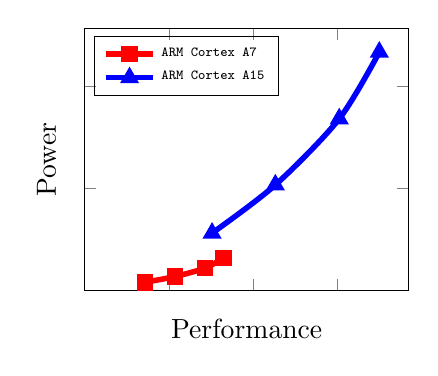
\begin{tikzpicture} %[>=latex]
\begin{axis}[
width=0.47\textwidth,
%line width=2,
%symbolic x coords={2012, 2013, 2014, 2015, 2016},
xticklabels={,,},
yticklabels={,,}
%xticklabels={720p,1080p,4k},
%minor xtick={0,1,...,18},
grid=both,
ymin=0,
xmin=0,
xlabel=Performance,
ylabel=Power,
legend pos=north west,
legend cell align=left,
legend style={
	font=\tiny,
	fill=none,
	%/tikz/column 2/.style={
	%	column sep=5pt,
	%},
},
%enlarge x limits=0.1,
%xticklabel style={text width=0.2\textwidth,align=flush left},
]
\addplot[line width=2pt,smooth,color=red,mark=square*] coordinates {
	(20/28,3/18)
	(30/28,5/18)
	(40/28,8/18)
	(46/28,11.5/18)
};
\addplot[line width=2pt,smooth,color=blue,mark=triangle*] coordinates {
	(42.3/28,20.3/18)
	(63.3/28,37.3/18)
	(84.5/28,60.6/18)
	(97.8/28,84.1/18)
};
\legend{\texttt{ARM Cortex A7~}\\\texttt{ARM Cortex A15}\\}
%\draw[red] plot [smooth] coordinates {(0 0) (2,3700) (4,6006) (18,18000)};
\end{axis}
\end{tikzpicture}
	%			%\includegraphics[width=0.46\linewidth]{fig/his-analysis/arm_cortex_a7_a15.jpg} 
	%		} 
	%		%\subfigure[Performance vs. power of nVIDIA CPUs.] { \label{fig:nvidia-pp-gtx} 
	%		%	\includegraphics[width=0.50\linewidth]{fig/his-analysis/gtx_gpu.jpg} 
	%		%}
	%		\subfigure[Performance vs. power of nVIDIA CPUs.] { \label{fig:nvidia-pp-gtx} 
	%			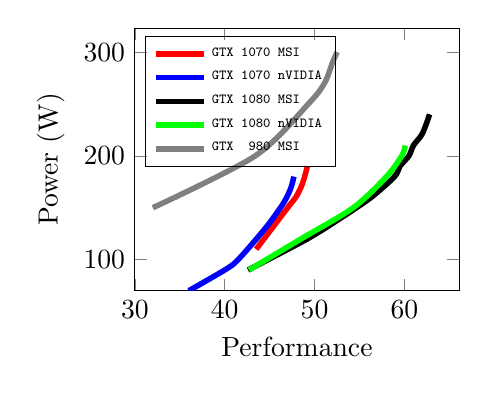
\begin{tikzpicture} %[>=latex]
\begin{axis}[
width=0.47\textwidth,
%line width=2,
%symbolic x coords={2012, 2013, 2014, 2015, 2016},
%xticklabels={,,},
%yticklabels={,,}
%xticklabels={720p,1080p,4k},
%minor xtick={0,1,...,18},
grid=none,
xmin=30,
ymin=70,
xlabel=Performance,
ylabel=Power (W),
legend pos=north west,
legend cell align=left,
%legend columns=2, 
legend style={
	font=\tiny,
	fill=none,
	%/tikz/column 2/.style={
	%	column sep=5pt,
	%},
},
%enlarge x limits=0.1,
%xticklabel style={text width=0.2\textwidth,align=flush left},
]
\addplot[line width=2pt,smooth,color=red] coordinates {
	(43.5,110) (47,150) (47.9,160) (48.5,170) (48.9,180) (49.2,190)
};
\addplot[line width=2pt,smooth,color=blue] coordinates {
	(36,70) (40,90) (41.5,100) (44.5,130)
	(46.2,150) (46.9,160) (47.4,170) (47.7,180)
};
\addplot[line width=2pt,smooth,color=black] coordinates {
	(42.6,90) (49.2,120) (52.9,140) (56.3,160) (58.9,180) (59.5,190)
	(60.5,200) (61.0,210) (61.9,220) (62.4,230) (62.8,240)
};
\addplot[line width=2pt,smooth,color=green] coordinates {
	(42.7,90) (48.5,120) (54.3,150) (58.0,180) (59.7,200) (60.1,210)
};
\addplot[line width=2pt,smooth,color=gray] coordinates {
	(32.0,150) (43.4,200) (49.3,250) (51.1,270) (52.0,290) (52.5,300)
};
\legend{\texttt{GTX 1070 MSI}\\\texttt{GTX 1070 nVIDIA}\\\texttt{GTX 1080 MSI}\\\texttt{GTX 1080 nVIDIA}\\\texttt{GTX ~980 MSI}\\}
%\draw[red] plot [smooth] coordinates {(0 0) (2,3700) (4,6006) (18,18000)};
\end{axis}
\end{tikzpicture}
	%		}
	%		\caption{Performance vs. power of CPUs and GPUs.} 
	%		\label{fig:performance-power-cpus-gpus} 
	%\end{figure}
	\begin{figure}[ht]
		\begin{minipage}[t]{.50\linewidth}
			\centering
			\input{fig/his-analysis/arm-cortex-cpu2}
			\centerline{\parbox[t]{\linewidth}{\centering\footnotesize (a) Performance vs. power of ARM CPUs.}}
		\end{minipage}
		\hfill
		\begin{minipage}[t]{.50\linewidth}
			\centering
			\input{fig/his-analysis/gtx-gpu2}
			\centerline{\parbox[t]{\linewidth}{\centering\footnotesize (b) Performance vs. power of nVIDIA CPUs.}}
		\end{minipage}
		\caption{Performance vs. power of CPUs and GPUs.}
		\label{fig:performance-power-cpus-gpus} 
	\end{figure}
	
	Blem {\em et al.}~\cite{Blem:2015:ISA} did comprehensive benchmark tests over multiple commodity ARM, x86, and MIPS CPUs. Figure~\ref{fig:power-performance-isa} shows some of their results. 
	\begin{figure}[ht] 
		\centering 
		\subfigure[Tech-independent average power normalized to A8.] { \label{fig:tech-independent-avg-power} 
			\includegraphics[width=0.44\linewidth]{fig/his-analysis/avg-power_to_a8.png} 
		} 
		\subfigure[Power performance tradeoffs.] { \label{fig:power-performance-tradeoffs} 
			\includegraphics[width=0.52\columnwidth]{fig/his-analysis/power-performance_tradeoffs.png} 
		}
		\caption{Power and performance of different CPU architectures.} 
		\label{fig:power-performance-isa} 
	\end{figure}
	
	If we replace the lateral axis to cost in monetary units, the curve will remain a similar shape. 
	
	Usually, cloud uses high-performance chips while fog uses low-power ones. If we can achieve near-linearly scaling, fog surely will be more cost and energy efficient. 
	
	\item The problems of distributed power generation are ``hard'', while ``soft'' in fog.\\
	To integrate with the grid and interoperate with other systems, there are problems like synchronisation and voltage control remaining to be solved. All of them require replacement of hardware. In contrast, most fog problems lie in the software layer and can be easily solved by complying with unified protocols. 	
	\item Interoperability.\\
	Due to rate, frequency, voltage, availability, reliability and operational management issues, integrating distributed generation to the electricity grids has always been a non-easily solvable issue.  
	\item The desirability of distributed generation is much weaker than that of fog computing.\\
	Recent technologies like UHV (Ultra-High-Voltage) electricity transmission have heavily reduced the desirability of distributed generation. However, because of the RTT-throughput relationship and fog's inherent proximity to the sensors at a local environment, the demand for fog computing keeps growing. 
	
\end{enumerate}

Therefore, it is clear that expectations regarding the future of distributed computing should not be based on the history of distributed generation.  
% http://www.greentechmedia.com/articles/read/the-energy-blockchain-could-bitcoin-be-a-catalyst-for-the-distributed-grid
%http://www.forbes.com/sites/williampentland/2016/06/27/bracing-for-blockchain-distributed-ledgers-poised-to-drive-adoption-of-distributed-generation/

\section{CCN and ICN}\label{sec:icn}
Historically, compared with servers and PCs, routers have usually had smaller memory. This has been due to cost considerations as well as properties of the Internet:
\begin{enumerate}
	\item The ``store-and-forward'' nature of the Internet infrastructure.\\
	The Internet was designed and built on top of existing telecommunication systems. In telecommunications, the ``store-and-forward'' principle and technique had been applied almost everywhere. 
	\item The packet loss rate does not improve much as the buffer size keeps increasing.\\
	The packet loss rate (which is simply equal to buffer overflow probability in most cases) is a negative exponential function of the buffer size. 
	From Anick's \cite{Anick1982Stochastic} and Guerin's \cite{Guerin1991Equivalent} works, it is not hard to derive Equation~\ref{eq:packet-loss-rate}, which satisfies both the finite and the infinite buffer assumption models, just with different values of $A$. 
	\begin{equation}\label{eq:packet-loss-rate}
	\epsilon \approx A\mathrm{e}^{-Bx}
	\end{equation}
	where $\epsilon$ is the loss rate and $x$ is the buffer size. 
	
	Therefore, according to these theories, the buffer memory requirement of routers does not increase much with upgrades in QoS level or link capacity. 
\end{enumerate}
	As the primary usage of the Internet has transformed from host-centric, end-to-end communication (to find the address of a host in order to fetch certain data) to content retrieval (no matter where the data is), the traditional TCP/IP model has become more and more inefficient. Attempts to improve the model without changing the substrates have merely complicated things, as they have introduced ``patching-over-patching'' requirements. The advent of CDN was just one such example. Thus, in recently years, researchers have proposed Information-Centric Networking (ICN) \cite{Xylomenos2014ICN} architectures, such as Content-Centric Networking (CCN) \cite{Perino:2011:CCN}. In these architectures, information is the focal point, and it is named and decoupled with location. All routers (intermediate nodes) along the transmission paths deterministically cache, manage, and replace the transmitted data, thus improving the content retrieval efficiency and network resource utilisation in a transparent, ubiquitous, and fine-grained way for the receivers. 
	
	It is believed by many researchers that these models might revolutionise the Internet infrastructure in 15 years, although with significantly challenging difficulty and the prerequisite of replacing all current routers. 
	
	The understanding is that routers in these architectures shall be equipped with large memory size and large storage capacity in order to handle increased responsibilities. 
	
	Before the potential adoption of ICN, the advent of smart routers (see Section~\ref{sec-smart-routers}) suggests that in the future even most edge routers would be powered with large buffering or storage capacities. 
	
    Furthermore, we believe that our ``Pear Fog CDN'' will be one small step towards ICN. 

\section{WebRTC} % Web Evolutions
In June 2011, about one year after acquiring Global IP Solutions (GIPS), Google released an open source project containing some of its core technologies for browser-based real-time communication known as Web Real-Time Communication (WebRTC). On-going standardisation work has been followed by W3C (as WebRTC, for browser APIs) and IETF (as RTCWeb, for substrate protocols). 

The advent of WebRTC just brings the real-time communication technology and application to the Web front-end; it provides browsers and mobile applications with peer-to-peer media streaming and data communication capabilities via simple APIs and without any pre-installed/standalone third-party programs/SDKs. 

In fact, from one perspective WebRTC has killed the media engine industry, while from another angle WebRTC will create a new Over-The-Top (OTT) ecosystem that will thoroughly redefine communication. 

Figure~\ref{fig:web-evolution} depicts the evolution of the Web in browser working models. 
\begin{figure}[ht]
	\centering
	\includegraphics[width=0.75\textwidth]{fig/webrtc/web_evolution.pdf}
	\caption{Path to WebRTC: a Web evolution picture.}\label{fig:web-evolution}
\end{figure}

WebRTC basically has three groups of APIs exposed to Web browsers: 
\begin{description}
	\item[MediaStream] 
	-- acquisition of audio and video streams
	\item[RTCPeerConnection] 
	-- communication of audio and video data
	\item[RTCDataChannel] 
	-- communication of arbitrary data
\end{description}

Apart from live audio and video streaming and video conferencing, there have been creative uses of WebRTC in healthcare, online maps, Location-Based Services (LBS), FinTech, and IoT. Some professionals have even predicted that WebRTC will provide ultimate solutions for powering industrial networks with media streaming and Web integration and interoperation capabilities, as well as bringing real-time VR/AR abilities to browsers. 

Azevedo {\em et al.}~\cite{Azevedo:2015:API} proposed an API extension to enable WebRTC application to access sensor data and an architecture for exchanging the data among peers through SRTP or SCTP, bringing nearby sensor streams to browser/client applications and media communications. They believe that the Android OS should be the first target in prototype implementation because it presents the best support for WebRTC. 
Bille {\em et al.}~\cite{Bille:2016:RTCSS} proposed an extensible framework on top of WebRTC. They achieve data synchronisation between browsers using a publish/subscribe paradigm. A centralised signalling server is needed during the whole process. They contemplated not only functionality, ease-of-use, but also data privacy. Developers can realise their business logic basically in a Finite State Machine (FSM) fashion with overriding callback functions.

The first known proposal to fulfil the Browser CDN (``peer-assisted delivery'', ``serverless CDN'', or ``P2P CDN'') needs was Maygh \cite{Zhang2013Maygh}. However, it is still nothing but an idea, because when it was proposed in 2013, Google's WebRTC implementation could not deliver reliable, ordered, binary data through either SRTP or SCTP (DataChannel). Later on, Bu {\em et al.} devised PeerJS \cite{bu2013peerjs}, which wrapped a shim layer and mimicked TCP traffic in JavaScript. This project eventually becomes obsolete, because the hacks were no longer necessary, as Google's implementation of WebRTC specifications became more and more complete. 

Maybe just two years ago the biggest obstacle to the wide adoption of WebRTC was that neither Microsoft nor Apple seemed willing to support it. Now this obstacle has totally disappeared. Microsoft implemented the basic features of ORTC (WebRTC 1.1) to its Edge browser in June 2015; Apple hired an engineer \cite{apple-webrtc} and has started to add support for WebRTC in its WebKit since April 2016\footnote{\url{https://webkit.org/status/\#specification-webrtc}}. 

It is expected that the WebRTC market will reach USD 4.45 billion by 2020, at a compound annual growth rate (CAGR) of 51\% from 2015 to 2020 \cite{webrtc-market}. In 2015 more than USD 1 billion in funding went to WebRTC-related companies and over 40 mergers and acquisitions took place. Early adopters are expected to be the first to reap the rewards of this growth. 

Figure~\ref{fig:webrtc-timeline} illustrates the evolution to Pear's WebRTC-based CDN, along with the WebRTC browser support timeline.  
\begin{figure}[ht]
	\centering
	\includegraphics[width=1.00\textwidth]{fig/webrtc/webrtc_timeline.pdf}
	\caption{WebRTC supporting status and trials timeline.}\label{fig:webrtc-timeline}
\end{figure}

\section{Bitcoin, Blockchain, and Smart Contract}
Since 2009, we have witnessed a spontaneous experiment in currency, payment, trust and credit systems, driven by Bitcoin \cite{nakamoto2009bitcoin}. In spite of its applications, Bitcoin might be the first P2P system that has created a self-sustainable\footnote{Or even self-enforcement/self-reinforcement in a Nash Equilibrium view.} incentive. 

Bitcoin was designed to build a pure peer-to-peer electronic payment network that does not rely on any trusted third-party. The cause of this demand was the trust crisis of banks and governments since the financial crisis of 2007. To solve the biggest challenge of ``double-spending'' in electronic payment systems, Bitcoin developed a framework that firstly solves the transaction and the recording problems and then realises immutability (unchangeability), resulting in a cryptographic proof-based technique called Blockchain. 

Some people have said that Bitcoin is a failed experiment, due to:
\begin{itemize}
	\item the centralisation incurred by professional miners using Application-Specific Integrated Circuits (ASICs);\\
	Now over 70\% of the computing power is concentrated in a few mining pools in China. 
	\item the huge electricity consumed by miners;\\
	This has further brought in selling pressure. 
	\item  the complex conflict of interests; the division in the community, and the evacuation of core developers.\\
	Perhaps Bitcoin is just too close to money, which makes people too greedy. 
\end{itemize}

Nevertheless, the blockchain technology Bitcoin brought to the world is an exciting one that might be the biggest thing that will change the world since the commercialisation of the Web in the mid-1990s. A blockchain is essentially a public ledger of all transactions or a distributed database of records or digital events that have been executed and shared among participating parties \cite{blockchain-tech}. Each event in the database is verified by consensus of a majority of the participants in the system. The core concept is essentially a consensus mechanism that records what happened at what time. Some famous VC investors, like Marc Andreessen, compare it to previous tech revolutions: Personal computers in 1975 and the Internet in 1993. They even believe that blockchain's distributed consensus model is the most important invention since the Internet itself. The Internet has facilitated the propagation of information; the blockchain will actualise the transfer of value. 

The attributes of blockchain further inspired something bigger than a digital cryptocurrency --- a smart contract, which incrementally adds ``additional conditions'' that can be executed on every peer automatically. Ethereum\footnote{\url{https://www.ethereum.org/}} is a blockchain-based distributed computing platform that accomplishes this job. It implements a Turing-complete language that can be used to create ``contracts'' that can be used to encode arbitrary state transition functions (to EVM Bytecode), allowing users to create systems to fulfil contract applications like exotic options. 

By September 2014, Ethereum had crowd-funded over USD 18 million, merely with an open source software project. The DAO, a decentralised autonomous organisation, instantiated on the Ethereum blockchain, raised over USD 150 million recently within 28 days, making it the world's largest crowd-funding project in history. On 17 June 2016, The Dao endured a real-time theft of about USD 50 million worth of \emph{ether}. The hacker said he was simply taking advantage of a technical loophole\footnote{It is a bug in the smart contract program, and not in the Ethereum platform itself.}. Although the chain was successfully hard-forked\footnote{With the support from over 85\% of the miners.} at last, and the crowd-funded money was returned to the volunteers on 21 July, the heist has caused people to rethink the experiment. It exposed the inevitability of human weakness, and reversely proved that it is humanity that is making the beautiful dreams possible, not necessarily mathematics. 
%http://dl.acm.org/citation.cfm?id=2813659&dl=ACM&coll=DL&CFID=651202385&CFTOKEN=28769825#URLTOKEN#

Blockchains have the potential to monetise transactions, proofs of work, verifications, and notarisations. But its too-close-to-money attribute may arouse people's greed to betray their peers and destroy what started as a beautiful idea. Recently, a group of researchers proposed DDoSCoin \cite{ddoscoin}, which is a cryptocurrency with a malicious proof-of-work. It helps to identify when a large number of connections via TLS have been made from a miner to a victim site. This further exposes the ugliness of some humans' hearts. 

%http://scet.berkeley.edu/wp-content/uploads/BlockchainPaper.pdf
The blockchain technology can be seen as a tool that could prove the existence and exact content of any data or digital asset at a particular time. It is an integration and automation of human-machine interaction and the Machine-to-Machine (M2M) and IoT payment network for the machine economy. Remember the distributed generation we discussed in Section~\ref{sec-dg-vs-dc}?  Although the desirability for distribution generation is weak, emerging domain-specific adoption of blockchain technology \cite{dg-blockchain} may bring distributed generation to some homes. We still have not seen wide deployments, while we will keep an eye on it.

From the rises and falls of the Bitcoin price, we have also learned that if a person puts his or her digital currency (token money) into the free market for trading, he or she should get ready for a roller coaster ride. Sometimes, there can even be a ``tulpenmanie''. 

\section{Development of Hardware}\label{sec-dev-hardware}
In the past few years, we have witnessed the explosive growth of edge devices, as well as their utilities and functionalities. These have greatly influenced Pear's business strategy. 

\subsection{IoT and Wearable: Barrier and Standardisation}
In the past few years, many people have swarmed into the field of wearable devices. However, we have also witnessed a falling of the tide.  
For wearables, the bottleneck is the batteries, which require a significant breakthrough in another domain, which is not predictable. Pear does not intend to penetrate this technology or business too early. 

On 13 January 2014, Google acquired Nest for USD~$3.2$ billion. This acquisition triggered a swarm into the Smart Home concept. Although people have tried IoT for many years, Apple even emphasising it in late 1970s, the largest barrier to IoT's market penetration is the disunity in standard protocol adoption. Each manufacturer has used its own proprietary protocols and technologies and has been unwilling to be connected to (let alone controlled by) something from another vendor. The good news\footnote{The bad news is that when we eventually get what we want, we will not want what we get, as the Bible states that the entire Web will be controlled by an evil world leader, who will use it to punish, starve, or even kill people who do not want to follow him. Thus, freedom from IoT is actually a blessing at this time.} is that we are starting to see some moves towards standardisation. 

\subsection{Smart Routers}\label{sec-smart-routers}
On 23 April 2014, XiaoMi launched an OpenWrt-based smart Wi-Fi router with 1TB NAS. It was a landmark event that motivated a lot of hardware vendors as well as Internet software service companies to crowd into this market. Lenovo introduced NewWiFi, also on top of OpenWrt. Huawei released Honor Router, which runs a proprietary version of embedded Linux. Google announced OnHub, which runs Chrome OS. All the three became ``phenomenal products''. 
They have tried to penetrate the market with smart Wi-Fi routers due to two main factors:
%in hope of ``future proofing''. Following their logic, 
\begin{enumerate}
	\item Wireless routers are entry points of users' data traffic;
	\item Wireless routers are control centres in smart homes.
\end{enumerate}

Basically, they see the trend of IoT and want a slice of the pie. Unfortunately, there is still no evidence showing that any of them has successfully built a sustainable ecosystem. Some reports have even stated that they did it too early and will just ``miss the rally'' in this field\footnote{\url{http://digi.tech.qq.com/a/20160621/006635.htm}}. 
% [xxx maybe more?...]

In our view, the root cause is that the current smart routers are not developer-friendly. Here is our reasoning:
\begin{enumerate}
	\item Neither OpenWrt nor embedded Linux is an easy platform for application development; 
	\item Because developing apps on/for such systems has a steep learning curve, there are few developers working on these platforms; 
	\item As there are few developers, there are few apps;
	\item As a result of the paucity of apps, there are few attractive features to users; 
	\item Since there are few compelling, needed features, users would rather buy a cheap USD~$10$ router.
\end{enumerate}

What a negative feedback loop! In most of IT history, any platform that captured a market was usually able to do so because it won the developers beforehand. 

However, we have now reached a turning point. MediaTek (MTK), the fourth largest fabless IC designer in the world has been powering its Wi-Fi router SoCs with the ARM Cortex architecture, which is the same as that of the CPUs used in most smartphones, tablets and TV-boxes. See Table~\ref{tb:mtk-soc}\footnote{For more information, pay attention to a relatively complete list of their change of chip architecture with time: \url{https://wikidevi.com/wiki/MediaTek}.}.
\begin{table}[htbp]
	\centering
	\caption{Wi-Fi Router SoC Evolution of MTK (MediaTek).}\label{tb:mtk-soc}
	\begin{tabular}[t]{llrrr}  
		\toprule
		SoC & Architecture  & Clock Speed & Cores & Release Time\\
		\midrule
		MT7620A/N	& MIPS 24KEc & $580/600$ MHz & 1 & Q1 2013\\
		MT7688A/K	& MIPS 24KEc & $575/580$ MHz & 1 & Q4 2014\\
		MT7628A/N	& MIPS 24KEc & $575/580$ MHz & 1 & Q2 2015\\
		MT7621A     & MIPS 1004Kc & $880$ MHz    & 2 & Q2 2014\\
		MT7621S     & MIPS 1004Kc & $880$ MHz    & 1 & Q4 2014\\
		MT7623A/N   & ARM Cortex A7	& $1.3$ GHz	 & 4 & Q2 2015\\
		MT7623N	    & ARM Cortex A7	& $1.3$ GHz	 & 4 & Q2 2015\\
		MT7683	    & ARM Cortex A7	& $1.3$ GHz	 & 4 & Q3 2015\\
		\bottomrule
	\end{tabular}
\end{table}

From a partner company specialising in ODM solutions for routers, we have learned that MTK has launched a new wireless chipset product-line\footnote{\url{http://www.mediatek.com/en/products/connectivity/wifi/home-network/wifi-ap/mt7623na/}} using the said ARM architecture. In addition, they planned to release the first Wi-Fi router demo solution running an Android OS in August 2016. 

Combining the above information and some business considerations, we have decided to produce and sell our all-in-one Pear smart router in a crowd-funding way. In short, it is a [Wi-Fi router] + [TV-box] + [PC] + [Sensor hub].  

In the Cloud, it is an access point working at the edge; in Home Entertainment, it is a media centre; in the IoT, it is a controller of all sensors; in the Fog, it is a member of the distributed service pool. 

Briefly speaking, a fog node is a micro data centre that descends the intelligence and resources from the core to the edge of the Internet, enabling the innovative capabilities to provide novel and refined applications and services.  

\subsection{Larger Memory and Storage at Lower Prices: A Continuous Trend} % comes together with CCN and ICN section??

In August 2015, Intel announced its 3D XPoint\footnote{\url{http://www.intel.com/content/www/us/en/architecture-and-technology/3d-xpoint-unveiled-video.html}} technology, which can achieve 1,000x higher performance and 1,000x longer endurance than the current NAND Flash and 10x storage density than DRAM. In the first real demo \cite{intel-3dxpoint-ssd}, each channel offered 6GB/s of I/O bandwidth. As more and more Storage Class Memory (SCM) implementations surface, we expect to continuously witness the prices of NAND Flash chips and HDD drives plummeting. 

Please also keep in mind that the DRAM costs are dropping about 32\% every 12 months. These would be a support for bringing large buffering, caching, and storage capacity to edge devices, helping realise ICN (as introduced in Section~\ref{sec:icn}) as well. This should mean that our Pear smart router will become more and more competitive in performance and price and not a hindrance to user acceptance. 

%\subsection{Performance Per Dollar}
 
\newpage
